% !TeX root = ../proyecto.tex

\chapter{Desarrollo Experimental}\label{ch:desarrollo-experimental}
En este capítulo se exponen los experimentos realizados, los ajustes implementados en los algoritmos y los resultados
obtenidos en los distintos escenarios evaluados.
El objetivo principal fue analizar el rendimiento de los modelos entrenados con conjuntos de datos reducidos,
seleccionados mediante algoritmos meméticos y evolutivos.

\section{Datasets utilizados}\label{sec:datasets}
En el aprendizaje profundo, los datasets son colecciones de datos etiquetados o no etiquetados que se utilizan para
entrenar modelos.
Estos conjuntos de datos contienen ejemplos organizados que representan la entrada para el modelo y, en muchos casos,
también las etiquetas correspondientes que indican la salida deseada.
Los datasets varían en tamaño, calidad y tipo, dependiendo de la tarea a resolver, como la clasificación de imágenes,
el reconocimiento de patrones o la predicción de series temporales.


A continuación, se van a explicar cada uno de los Datasets que se han utilizado en el desarrollo del proyecto.

\subsection{Rock, Paper, Scissors (Piedra, Papel, Tijera)}\label{subsec:rock-paper-scissors}
\textbf{Rock, Paper, Scissors}~\cite{noauthor_rock_nodate} es un conjunto de datos creado por Laurence Moroney
que se utiliza para la clasificación de imágenes de manos representando los gestos de `piedra', `papel' y `tijeras'.

\subsubsection{Estructura del Dataset}
El conjunto de datos contiene aproximadamente 2,500 imágenes, distribuidas en tres categorías: piedra, papel y tijeras.
Las imágenes están en color y tienen un tamaño de 300x300 píxeles.

Las imágenes están organizadas en directorios según su categoría artística:
\begin{verbatim}
+-- train
|   +-- rock
|   |   +-- image1.jpg
|   |   +-- image2.jpg
|   |   \-- ...
|   +-- paper
|   |   +-- image1.jpg
|   |   +-- image2.jpg
|   |   \-- ...
|   \-- scissors
+-- test (originalmente valid)
|   +-- rock
|   +-- paper
|   \-- scissors
+-- valid (originalmente test)
|   +-- rock
|   +-- paper
|   \-- scissors
\end{verbatim}


\subsubsection{Formato de los Datos}
Las imágenes están en formato JPEG (\texttt{.jpg}). Para su procesamiento, se han aplicado técnicas de preprocesamiento
adaptadas a los requerimientos del modelo.

\subsubsection{Uso del Dataset}
Este dataset se ha utilizado para evaluar el rendimiento del modelo en un problema de clasificación de imágenes con
múltiples clases, pero siendo un dataset sencillo y con un número de clases pequeño.
Además, permite explorar la eficacia de los algoritmos meméticos en un entorno más cercano al reconocimiento de objetos.

\subsubsection{Correcciones en la División de Datos}
Según la nota observada en el README del dataset:
\begin{quote}
    \textit{Note: in the source, Laurence calls ``validation'' as the ``test'', and ``test'' the ``validation''.}
\end{quote}
se han renombrado las particiones de \texttt{test} y \texttt{valid} para que correspondan correctamente con sus
propósitos.

\subsubsection{Licencia y uso}
Este conjunto de datos se distribuye bajo la licencia
\textbf{Creative Commons Attribution 4.0 International (CC BY 4.0)}, lo que permite su uso, modificación y distribución
con la condición de otorgar el crédito adecuado a los creadores originales~\cite{moroney_laurence_nodate}.


\subsection{PAINTING (Art Images: Drawing/Painting/Sculptures/Engravings)}\label{subsec:painting}
El dataset \textbf{Art Images: Drawing/Painting/Sculptures/Engravings} es una colección de aproximadamente 9,000
imágenes organizadas en cinco categorías de arte: dibujos, pinturas, esculturas, grabados y arte iconográfico.

\subsubsection{Estructura del Dataset}
Las imágenes están organizadas en directorios según su categoría artística:
\begin{verbatim}
+-- Train (originalmente training_set)
|   +-- drawings
|   |   +-- image1.jpg
|   |   +-- image2.jpg
|   |   \-- ...
|   +-- paintings
|   |   +-- image1.jpg
|   |   +-- image2.jpg
|   |   \-- ...
|   +-- sculptures
|   +-- engravings
|   \-- iconography
+-- Test (originalmente validation_set)
|   +-- drawings
|   +-- paintings
|   +-- sculptures
|   +-- engravings
|   \-- iconography
\end{verbatim}

\subsubsection{Formato de los Datos}
Todas las imágenes están en formato JPEG (\texttt{.jpg}) y presentan variaciones en resolución y dimensiones.
Se han aplicado técnicas de preprocesamiento para homogenizar las características de las imágenes.

\subsubsection{Uso del Dataset}
Este dataset se ha utilizado para entrenar y evaluar modelos de clasificación de imágenes en un entorno diferente al
RPS\@.
Con este dataset, se ha comprobado el funcionamiento para evaluar los algoritmos con un dataset un poco mas complejo
que el RPS, con un par de clases más y con un número mayor de imágenes.

\subsubsection{Correcciones en la División de Datos}
Observando los tamaños de la división de los datos, y teniendo en cuenta que la divisón de los datos suele ser en train
y test, se ha decidido por renombrar las particiones de \texttt{valid} por \texttt{test} para que corresponda
correctamente con su propósito.
Y el set de validation lo he obtenido separando el set de train, normalmente haciendo una división 80\% test y 20\%
valid.

\subsubsection{Acceso al Dataset}
Inicialmente, el dataset se descargó desde Kaggle~\cite{noauthor_original_nodate}

Sin embargo, debido a la presencia de archivos innecesarios y algunas imágenes corruptas, se optó por una versión
limpia disponible en Kaggle~\cite{noauthor_cleaned_nodate}.

\subsubsection{Licencia y Uso}
Antes de su uso, se revisaron los términos y condiciones establecidos en la página de Kaggle para asegurar el
cumplimiento con las licencias y restricciones aplicables.

\subsection{MNIST (Modified National Institute of Standards and Technology)}\label{subsec:mnist}
\textbf{MNIST}~\cite{noauthor_mnist_nodate} es un dataset ampliamente utilizado en aprendizaje profundo.
Contiene 70,000 imágenes de dígitos escritos a mano, divididas en 60,000 imágenes para el entrenamiento y 10,000 para
la prueba.

\subsubsection{Estructura del Dataset}
Las imágenes tienen un tamaño de 28x28 píxeles y están en escala de grises, con valores de intensidad entre 0 (negro) y
255 (blanco).

\subsubsection{Formato de los Datos}
Las imágenes están almacenadas en formato IDX, un formato binario específico para este dataset.
Se ha realizado una conversión a matrices NumPy para su procesamiento eficiente.

\subsubsection{Uso del Dataset}
Este conjunto de datos se ha empleado como benchmark para evaluar modelos de clasificación de imágenes, especialmente
en arquitecturas convolucionales.

\subsubsection{Licencia y uso}
El dataset MNIST se distribuye bajo una licencia de dominio público.
Fue creado a partir de los datos originales del NIST y está disponible en diversas plataformas, incluyendo la página
oficial de Yann LeCun~\cite{lecun_yann_nodate}.


\subsection{Comparación con otros datasets}\label{subsec:comparacion-con-otros-datasets}
\colorbox{yellow}{Aqui va una comparación de todos los datasets usados}
%La selección de estos dos datasets responde a la necesidad de evaluar los algoritmos meméticos en distintos niveles de
%complejidad.
%\textbf{MNIST}, con imágenes en escala de grises de bajo nivel de complejidad, proporciona una referencia clara y
%estandarizada para comparar el rendimiento y la reducción de datos.
%Por otro lado, el dataset de \textbf{Rock, Paper, Scissors} introduce más desafíos visuales y complejidades,
%permitiendo analizar cómo los algoritmos meméticos se comportan en escenarios más complejos que podrían ser
%representativos de aplicaciones más reales en visión por computadora.


\section{Diseño de los experimentos}\label{sec:diseño-de-los-experimentos}
La fase experimental se organizó en varias etapas.
Inicialmente se optó por un dataset simple (Rock, Paper, Scissors) para validar el funcionamiento general del sistema.
Posteriormente, se realizaron pruebas con datasets más exigentes, como PAINTING y MNIST. Los experimentos se repitieron utilizando
diferentes porcentajes iniciales de datos (10\%, 25\%, 50\% y 75\%) para estudiar cómo afecta la cantidad de datos seleccionados al rendimiento del modelo.

Con el fin de asegurar la consistencia entre ejecuciones experimentales, se aplicaron las medidas de control de reproducibilidad detalladas previamente en el \hyperref[sec:consideraciones-de-optimizacion]{Capítulo 6}.
Esto permitió comparar algoritmos en condiciones homogéneas, evitando variaciones indeseadas causadas por componentes aleatorios del entorno de ejecución.

En cada prueba, se realizaron cinco ejecuciones paralelas con semillas distintas.
Se calcularon las medias de las métricas más relevantes (accuracy, precision, recall y F1-score), junto con el tiempo de ejecución y número
de evaluaciones realizadas.

\section{Evaluación con modelos base}\label{sec:evaluacion-con-modelos-base}
Los primeros experimentos se realizaron con los algoritmos aleatorios, tanto en ResNet50 como en MobileNet, como línea base comparativa.
En ambos modelos, se observó una mejora gradual de las métricas al aumentar el porcentaje de datos utilizados.
Como era de esperar, ResNet50 ofreció mejores resultados en cuanto a precisión, pero a costa de un mayor tiempo de entrenamiento.
MobileNet, en cambio, ofreció una alternativa más rápida y eficiente, aunque con una leve pérdida de rendimiento.

\begin{table}[htp]
    \centering
    \resizebox{\textwidth}{!}{
        \begin{tabular}{lp{2cm}lp{2cm}p{2cm}p{2cm}p{2cm}p{2.2cm}}
            \toprule
            \textbf{Algoritmo}       & \textbf{Porcentaje Inicial} & \textbf{Duración}       & \textbf{Accuracy (Avg)} &
            \textbf{Precision (Avg)} & \textbf{Recall (Avg)}       & \textbf{F1-score (Avg)} &
            \textbf{Evaluaciones Realizadas}                                                                                                               \\
            \midrule
            \multicolumn{8}{l}{\textbf{Modelo ResNet50}}                                                                                                   \\
            \midrule
            aleatorio                & 10                          & 00:45:08                & 76,55\%                 & 81,80\% & 76,55\% & 76,25\% & 100 \\
            aleatorio                & 20                          & 01:10:27                & 81,77\%                 & 84,70\% & 81,77\% & 81,59\% & 100 \\
            aleatorio                & 50                          & 02:24:49                & 87,14\%                 & 88,09\% & 87,14\% & 86,97\% & 100 \\
            aleatorio                & 100                         & 00:02:42                & 87,90\%                 & 88,96\% & 87,90\% & 87,81\% & 1   \\
            \midrule
            \multicolumn{8}{l}{\textbf{Modelo MobileNet}}                                                                                                  \\
            \midrule
            aleatorio                & 10                          & 00:29:29                & 72,31\%                 & 76,40\% & 72,31\% & 69,62\% & 100 \\
            aleatorio                & 20                          & 00:50:36                & 76,48\%                 & 78,82\% & 76,48\% & 75,58\% & 100 \\
            aleatorio                & 50                          & 01:54:09                & 75,56\%                 & 79,72\% & 75,56\% & 74,67\% & 100 \\
            aleatorio                & 100                         & 00:02:12                & 76,08\%                 & 79,97\% & 76,08\% & 75,61\% & 1   \\
            \bottomrule
        \end{tabular}
    }
    \caption{Comparativa de resultados de la generación inicial utilizando el algoritmo \textbf{aleatorio} con los modelos \textbf{ResNet50} y \textbf{MobileNet}.}
    \label{tab:initial-generation-comparison}
\end{table}


En las Tabla~\ref{tab:initial-generation-comparison} se muestran los resultados obtenidos para diferentes porcentajes iniciales de datos con ambos modelos.
Además, en la Figura X se incluye un boxplot donde se comparan los valores de accuracy por porcentaje de datos y por algoritmo.

\section{Comparativa entre Algoritmos}\label{sec:comparativa-entre-algoritmos}
A lo largo del desarrollo del proyecto, se diseñaron y ajustaron diversas versiones de algoritmos evolutivos y meméticos para seleccionar subconjuntos representativos de imágenes. Esta sección presenta una comparativa entre ellos, no solo desde una perspectiva cuantitativa (accuracy, precisión, etc.), sino también cualitativa, incorporando los aprendizajes progresivos que guiaron su evolución.

\subsection{Iteración inicial: comparación base}\label{sec:iteracion-inicial-comparacion-base}
La primera comparativa se centró en tres enfoques principales:

\begin{itemize}
    \item \textbf{Algoritmo aleatorio}, como línea base sin criterio de selección.
    \item \textbf{Búsqueda local}, ajustando iterativamente el conjunto seleccionado.
    \item \textbf{Algoritmo genético (v1)}, combinando subconjuntos mediante operadores clásicos de cruce y mutación.
    \item \textbf{Algoritmo memético}, que combinaba el genético con un proceso de mejora local adicional.
\end{itemize}

\begin{figure}[!h]
    \centering
    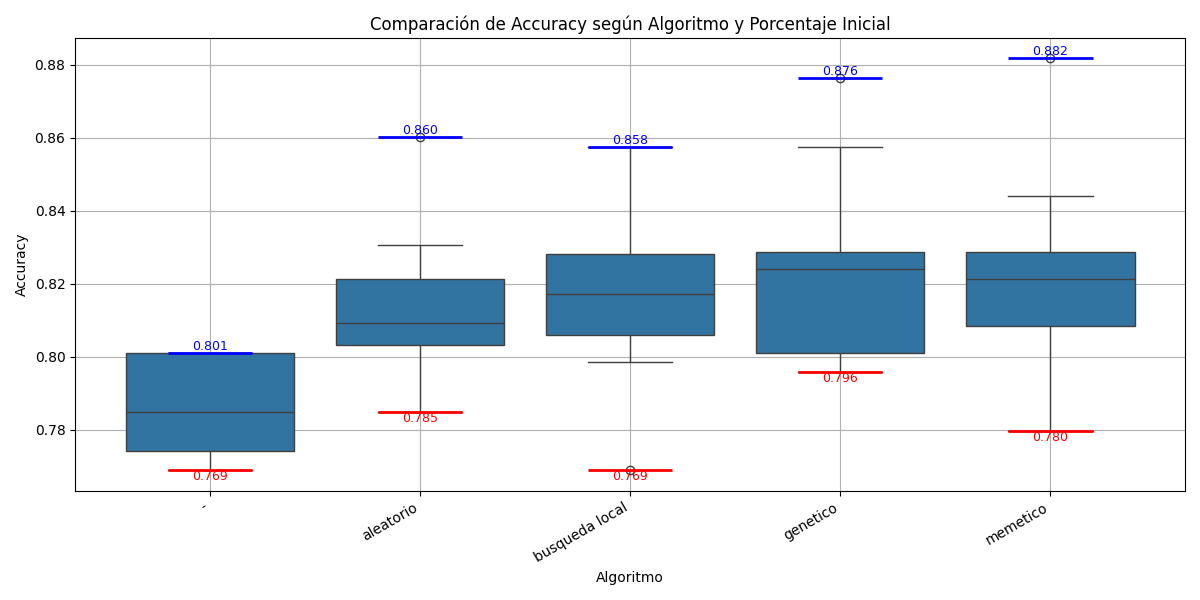
\includegraphics[width=0.95\textwidth]{imagenes/mobilenet-BOXPLOT-generacion-inicial}
    \caption{Boxplot comparando el \textit{accuracy} alcanzado por cada algoritmo de los iniciales.}
    \label{fig:boxplot-generacion-inicial}
\end{figure}

El gráfico de la Figura~\ref{fig:boxplot-generacion-inicial} ofrece una visión comparativa del rendimiento de los algoritmos evaluados en la etapa inicial del proyecto.
Se observa que el algoritmo aleatorio, como era de esperar, presenta una alta dispersión y una mediana de accuracy relativamente baja.
Este comportamiento se justifica por la ausencia de una estrategia que guíe la selección de datos, lo que da lugar a conjuntos de entrenamiento inconsistentes.


Por su parte, la búsqueda local mejora notablemente la mediana de accuracy, manteniendo una menor variabilidad que el enfoque aleatorio.
Esto indica que, pese a su simplicidad, la exploración guiada del espacio de soluciones permite alcanzar resultados más estables y competitivos.


El algoritmo genético (v1) representa un salto adicional en rendimiento.
La combinación de operadores evolutivos como la selección, el cruce y la mutación genera soluciones más refinadas,
lo que se traduce en una mediana superior y en una mayor compactación de los valores en torno a ella.


Finalmente, el algoritmo memético destaca como el más eficiente dentro de esta primera iteración.
Al incorporar una fase de mejora local sobre la evolución genética, logra afinar aún más las soluciones obtenidas.
Este enfoque híbrido permite reducir la dispersión y minimizar la probabilidad de obtener soluciones poco efectivas.


\subsection{Mejoras progresivas: evolución del algoritmo genético}\label{sec:mejoras-progresivas-evolucion-algoritmo-genetico}
Aunque el algoritmo memético alcanzó el mejor resultado puntual en la comparativa inicial, se decidió continuar el desarrollo
sobre el algoritmo genético por varias razones estratégicas.


En primer lugar, el análisis detallado mostró que el genético también presentaba una mediana de accuracy más alta,
lo que sugiere un rendimiento más consistente.
Además, incluso en sus ejecuciones menos favorables, el genético mostró mejores valores mínimos que el memético,
lo cual evidencia una mayor robustez frente a escenarios menos óptimos.


A nivel práctico, el algoritmo genético ofrecía una estructura más simple y modular, lo que facilitó la introducción progresiva de mejoras específicas.
Esta simplicidad también implicaba una menor carga computacional al prescindir de la búsqueda local en cada iteración,
permitiendo realizar pruebas más rápidas y escalables.
Por estos motivos, se consideró que centrar los esfuerzos en afinar el genético aportaría beneficios significativos
tanto en eficiencia como en estabilidad, sin renunciar a un rendimiento competitivo.


Por lo tanto, se optó por implementar varias versiones del algoritmo genético, cada una con mejoras específicas:


\begin{itemize}
    \item \textbf{Versión 2 (Genético v2)}: se introdujo un cruce ponderado que daba más peso al progenitor con mejor fitness,
          y se seleccionaba únicamente el mejor de los dos hijos generado.
          Esto evitaba la propagación de soluciones poco efectivas y mejoraba la velocidad de convergencia.
    \item \textbf{Versión 3 (Genético v3)}: se añadió una lógica de reinicio poblacional. Si después de varias generaciones
          no se observaba mejora, se mantenía el mejor individuo y se regeneraban aleatoriamente los demás.
          Esta estrategia ayudó a salir de óptimos locales sin reiniciar todo el proceso.
          % \item \textbf{Versión 4 (Genético v4)} [prototipo]: se exploró la posibilidad de conservar un histórico de las mejores
          %       soluciones y reutilizarlas en futuras generaciones como una forma de memoria evolutiva.
\end{itemize}

Estas versiones se probaron bajo las mismas condiciones que los algoritmos iniciales, lo que permitió compararlos en igualdad de condiciones.


Durante el desarrollo de la Versión 2, se evaluaron distintas estrategias para el operador de mutación.
Inicialmente, se aplicaba una regla fija que realizaba un 10\% de permutaciones sobre el subconjunto seleccionado:
\[
    \mathrm{num\_swaps} = \max\left(1,\ \mathrm{length} \times 0.1\right)
\]
Sin embargo, esta estrategia podía resultar demasiado conservadora o agresiva, según el tamaño de la solución.
En la versión final se adoptó una fórmula más flexible que adapta la magnitud de la mutación en función tanto del subconjunto mutado como del original:
\[
    \mathrm{num\_swaps} = \min\left(\mathrm{length} \times 0.15,\ \mathrm{length} \times 0.8\right)
\]
Esta modificación permite un equilibrio más eficaz entre exploración y preservación de estructura, limitando las perturbaciones excesivas sin eliminar la capacidad de escape de óptimos locales.

\colorbox{yellow}{Debe de comprobarse cómo funciona la fórmula con el ratio añadido:}
\[
    \mathrm{num\_swaps} = \min\left(\mathrm{length} \times 0.15,\ \mathrm{length} \times \mathrm{ratio} \times 0.8\right)
\]


\subsection{Evaluación de resultados}\label{sec:evaluacion-de-resultados}
A continuación, se presentan dos gráficos en forma de boxplot que comparan el rendimiento de los algoritmos con base en la métrica de \textit{accuracy}.
Estas visualizaciones permiten analizar la distribución de resultados, la variabilidad y la consistencia de cada enfoque:

\begin{figure}[!h]
    \centering
    
\includegraphics[width=0.95\textwidth]{imagenes/mobilenet-BOXPLOT-accuracy-porcentaje}
    \caption{Boxplot del \textit{accuracy} alcanzado por los algoritmos en función del porcentaje inicial de imágenes seleccionadas.}
    \label{fig:boxplot-accuracy-porcentaje}
\end{figure}

\begin{figure}[!h]
    \centering
    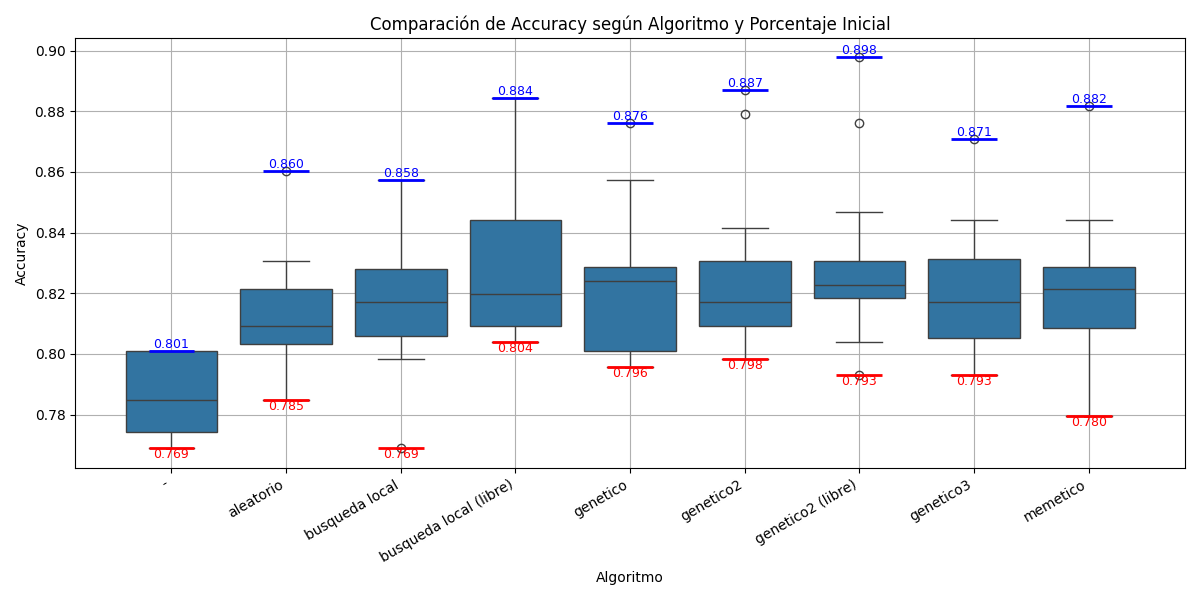
\includegraphics[width=0.95\textwidth]{imagenes/mobilenet-BOXPLOT-accuracy-algoritmo}
    \caption{Boxplot comparando el \textit{accuracy} alcanzado por cada algoritmo, agrupando los resultados según la estrategia utilizada.}
    \label{fig:boxplot-accuracy-algoritmo}
\end{figure}

\subsubsection{Análisis de los resultados}\label{sec:analisis-de-los-resultados}

El primer boxplot (Figura~\ref{fig:boxplot-accuracy-porcentaje}) muestra que, como era esperable,
el \textit{accuracy} mejora progresivamente al incrementar el porcentaje de datos usados.
Sin embargo, también se observa que algunos algoritmos, como los genéticos mejorados, obtienen valores muy competitivos
incluso con bajos porcentajes iniciales, lo que refuerza su utilidad como técnica de reducción.


En el segundo boxplot (Figura~\ref{fig:boxplot-accuracy-algoritmo}), permite comparar directamente el impacto de cada estrategia.
Las versiones mejoradas del algoritmo genético (v2 y v3), así como el algoritmo memético,
no solo alcanzan medianas de accuracy más altas, sino que también muestran menor variabilidad.
Esta menor dispersión indica una mayor estabilidad entre ejecuciones, lo cual es deseable en procesos
de optimización con componentes estocásticos.


Además, se observa una clara reducción en los valores atípicos negativos en los algoritmos mejorados, lo que sugiere una menor
probabilidad de obtener resultados significativamente bajos.
Esto es especialmente relevante en contextos donde se busca fiabilidad en entornos con recursos limitados.


En conjunto, los resultados evidencian que las mejoras introducidas, como el cruce ponderado, la lógica de reinicio poblacional
o la combinación con búsqueda local, aportan beneficios sustanciales en términos de rendimiento y robustez.
Estos algoritmos superan sistemáticamente a las estrategias más simples (aleatorio y búsqueda local), tanto en
precisión como en consistencia, confirmando su idoneidad para tareas de selección de subconjuntos de datos en aprendizaje profundo.


Estas observaciones permiten concluir que las modificaciones introducidas en el algoritmo genético no solo mejoran la media de rendimiento,
sino que también aportan consistencia y robustez frente a la aleatoriedad inherente a este tipo de procesos evolutivos.


\section{Análisis del balance de clases}\label{sec:analisis-del-balance-de-clases}
Adicionalmente, se realizó un análisis del balance de clases en las soluciones finales generadas por cada algoritmo.
El objetivo era comprobar si los subconjuntos seleccionados mantenían una representación equilibrada entre las
distintas clases del dataset (Paper, Rock y Scissors), o si ciertos algoritmos tendían a favorecer algunas clases frente a otras.


\begin{figure}[htp]
    \centering
    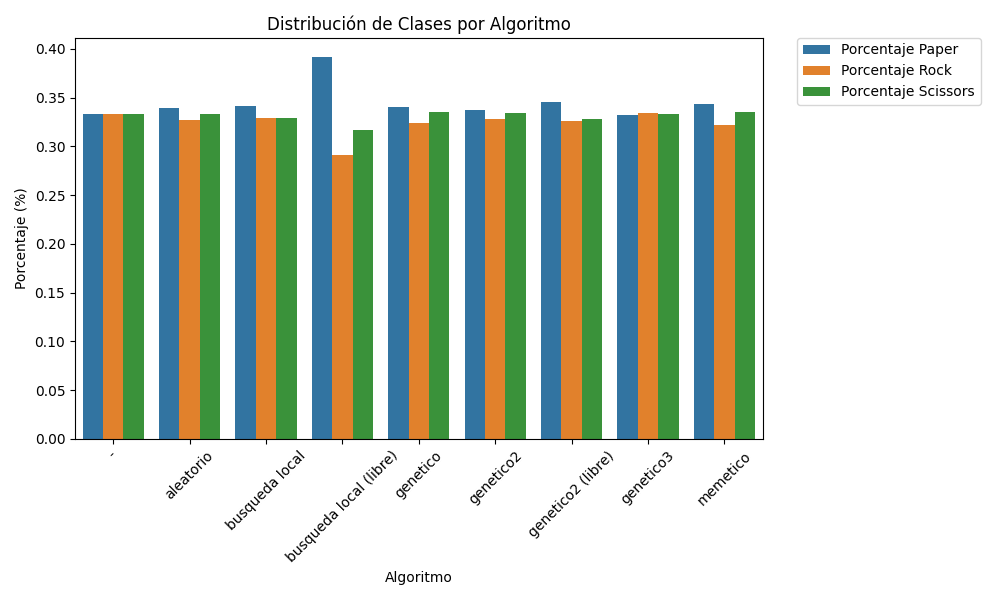
\includegraphics[width=1\textwidth]{imagenes/mobilenet-BARPLOT-balance-de-clases-por-algoritmo}
    \caption{Distribución del porcentaje de imágenes por clase en las soluciones generadas por cada algoritmo.}
    \label{fig:balance-de-clases-por-algoritmo}
\end{figure}

Tal como se observa en la Figura~\ref{fig:balance-de-clases-por-algoritmo}, los algoritmos más simples como el aleatorio o la búsqueda local presentan ligeras desviaciones, mientras que las versiones más avanzadas, en especial los algoritmos genéticos mejorados y el memético, logran mantener una distribución más homogénea entre clases.
Este equilibrio es clave para evitar sesgos en el modelo entrenado y mejorar métricas como el F1-score.


Aunque si podemos observar una leve tendencia a que los algoritmos necesitan unos pocos datos más de la clase \textit{Paper}, a la vez que reduce el porcentaje de la clase \textit{Rock}.


\begin{figure}[htp]
    \centering
    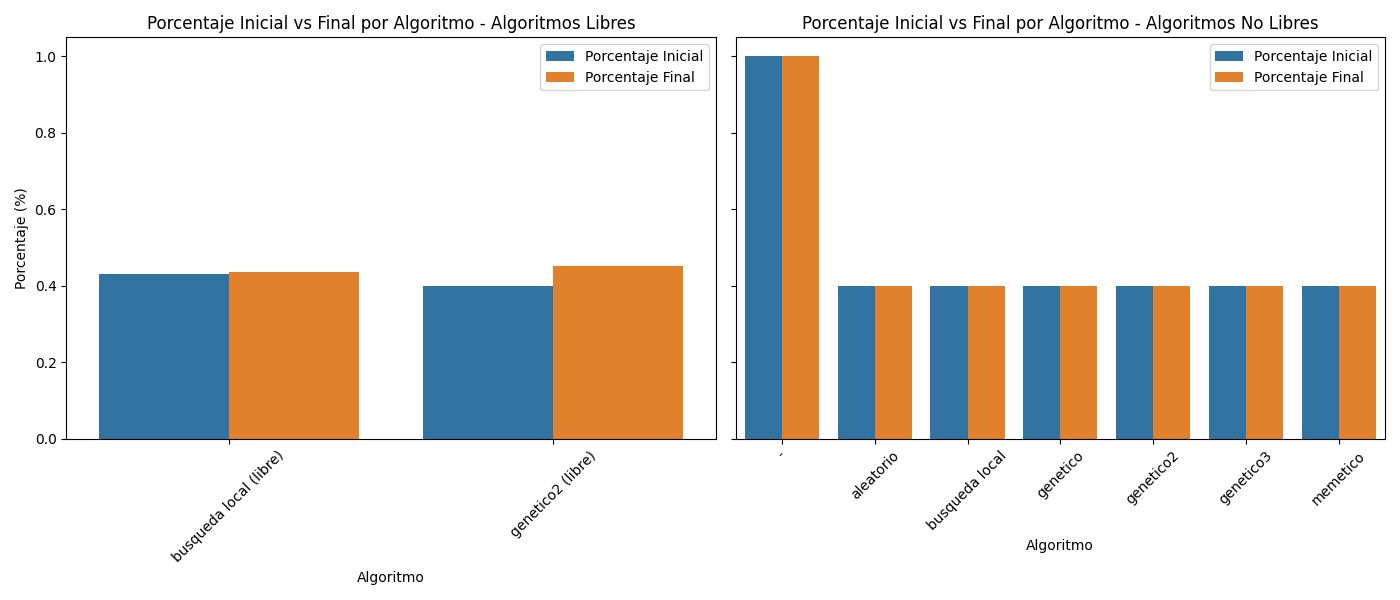
\includegraphics[width=1\textwidth]{imagenes/mobilenet-BARPLOT-porcentaje-inical-vs-final-por-algoritmo}
    \caption{Comparación entre porcentaje inicial y final de imágenes seleccionadas por algoritmo.
    }
    \label{fig:comparation-initial-final}
\end{figure}

Por otro lado, se analizó cómo varía el porcentaje de datos seleccionados desde el inicio hasta el final del proceso en cada algoritmo.
Este análisis, reflejado en la Figura~\ref{fig:comparation-initial-final}, permite observar si los algoritmos tienden a mantener,
reducir o incluso aumentar la cantidad de imágenes utilizadas durante su evolución.


Se puede apreciar que los algoritmos con un porcentaje fijo mantienen estable la cantidad de datos seleccionados, como era de esperar debido a su implementación.
Sin embargo, en los algoritmos con comportamiento “libre”, como \textit{búsqueda local (libre)} o \textit{genético2 (libre)}, si se observa su variabilidad,
en particular, ambos algoritmos tienden a aumentar el porcentaje de imágenes seleccionadas respecto al inicial,
lo que vuelve a confirmar la tendencia de necesitar más imágenes para mejorar el rendimiento del modelo.


\section{Validación con el dataset PAINTING}\label{sec:validacion-con-el-dataset-painting}
Para comprobar la generalización de los resultados, se repitieron los experimentos con el dataset PAINTING, de mayor tamaño y complejidad.
% En este caso, los mejores resultados también se obtuvieron con las versiones mejoradas de los algoritmos genéticos, seguidos muy de cerca por el memético.
% En todos los casos, se logró mantener o incluso mejorar el rendimiento del modelo en comparación con el uso del 100\% de los datos, empleando únicamente
% un subconjunto optimizado.

\colorbox{yellow}{Falta añadir el análisis detallado de los resultados obtenidos con el dataset PAINTING.}